\subsection*{Operations on sets}

We remember the important operations for sets:

\begin{itemize}
 \item $M_1 \cup M_2 := \{ x: x\in M_1 \vee x \in M_2 \}$ (union)
 \item $M_1 \cap M_2 := \{ x : x \in M_1 \wedge x \in M_2\}$ (intersection)
 \item $M_1 \setminus M_2 := \{ x : x \in M_1 \wedge x \not\in M_2 \}$ (set difference)
\end{itemize}

%$A \times B = \{ (a,b) : a \in A, b \in B\}$ the set of all 2-tuples
%From $\mathbb{R}\times \mathbb{R} = \{ (a,b): a,b \in \mathbb{R}\}$ there is only a short way to the 2d vector space.
%Missing: definition of addition and scaling. 
%
%A nice application in computer graphics is ``CSG'': Constructive Solid Geometry!


\begin{Definition}{Set compositions}
%\begin{figure}[htbp]
  \begin{minipage}[c]{0.5\textwidth}
  The \defi{union} $M_1\cup M_2$ 
  is the new set that consists exactly
  of the objects that are elements of $M_1$ \textbf{or} $M_2$.
  \end{minipage}
  \begin{minipage}[c]{0.4\textwidth}
  \flushright
     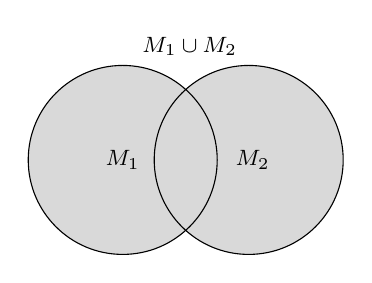
\begin{tikzpicture}[scale=0.8] % M_1 vereinigt M_2
\def\firstcircle{(0,0) circle (1.5cm)}
\def\secondcircle{(0:2cm) circle (1.5cm)}
    \draw[fill=black!15] \firstcircle node {\begin{footnotesize}$M_1$ \end{footnotesize}}
                  \secondcircle node {\begin{footnotesize} $M_2$ \end{footnotesize}};
    \node[anchor=south] at (current bounding box.north) {\begin{footnotesize} $M_1 \cup M_2$ \end{footnotesize}};
\end{tikzpicture}
  \end{minipage}
%\end{figure}
~\\[4ex]
%\begin{figure}[htbp]
  \begin{minipage}[c]{0.5\textwidth}
  The \defi{intersection} $M_1\cap M_2$ 
  is the new set
  whose elements 
  are the objects that are elements of $M_1$ \textbf{and} $M_2$.
  \end{minipage}
  \begin{minipage}[c]{0.4\textwidth}
  \flushright  
     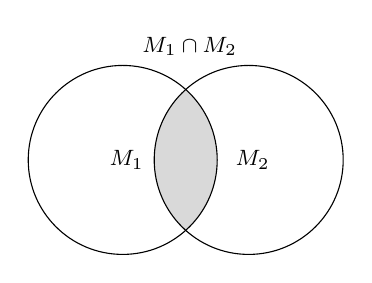
\begin{tikzpicture}[scale=0.8] % M_1 geschnitten M_2
\def\firstcircle{(0,0) circle (1.5cm)}
\def\secondcircle{(0:2cm) circle (1.5cm)}
    \begin{scope}
        \clip \firstcircle;
        \fill[fill=black!15] \secondcircle;
    \end{scope}
    \draw \firstcircle node {\begin{footnotesize} $M_1$ \end{footnotesize}};
    \draw \secondcircle node {\begin{footnotesize} $M_2$ \end{footnotesize}};
    \node[anchor=south] at (current bounding box.north) {\begin{footnotesize} $M_1 \cap M_2$ \end{footnotesize}};
\end{tikzpicture}
  \end{minipage}
%\end{figure}
~\\[4ex]
%\begin{figure}[htbp]
  \begin{minipage}[c]{0.5\textwidth}
  We write $M_1\setminus M_2$ 
  for the \defi{set difference}
  whose elements are the objects
  that are elements of $M_1$ \textbf{but not} elements of $M_2$.
  \end{minipage}
  \begin{minipage}[c]{0.4\textwidth}
  \flushright
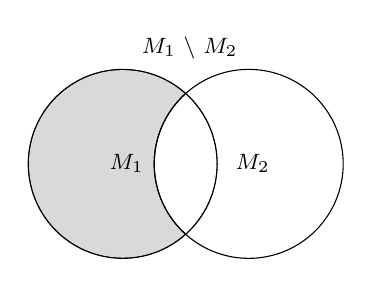
\begin{tikzpicture}[scale=0.8] % M_1 ohne M_2
\def\firstcircle{(0,0) circle (1.5cm)}
\def\secondcircle{(0:2cm) circle (1.5cm)}
    \begin{scope}
        \clip \firstcircle;
        \draw[fill=black!15, even odd rule] \firstcircle node  {\begin{footnotesize} $M_1$ \end{footnotesize}}
        \secondcircle;
    \end{scope}
    \draw \firstcircle
                   \secondcircle node {\begin{footnotesize} $M_2$ \end{footnotesize}};
    \node[anchor=south] at (current bounding box.north) {\begin{footnotesize} $M_1 \  \backslash \ M_2$\end{footnotesize}};
\end{tikzpicture} 
  \end{minipage}
%\end{figure}
~\\[4ex]
%\begin{figure}[htbp]
  \begin{minipage}[c]{0.5\textwidth}
  A \defi{subset} of $M_2$
  is each set whose elements are also elements of $M_2$.
  \end{minipage}
  \begin{minipage}[c]{0.4\textwidth}
  \flushright
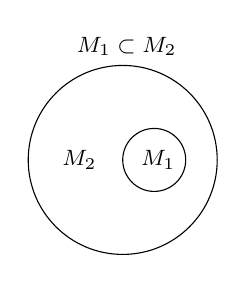
\begin{tikzpicture}[scale=0.8]
\def\firstcircle{(0,0) circle (1.5cm)}
\def\secondcircle{(0:0.5cm) circle (0.5cm)}
    \begin{scope}
        %\clip \firstcircle;
        \draw \firstcircle node at(-0.75,0) {\begin{footnotesize} $M_2$ \end{footnotesize}};
        \secondcircle;
    \end{scope}
    \draw \secondcircle node {\begin{footnotesize} $M_1$ \end{footnotesize}};
    \node[anchor=south] at (current bounding box.north) {\begin{footnotesize} $M_1 \subset M_2$\end{footnotesize}};
\end{tikzpicture} 
  \end{minipage}
%\end{figure}
\end{Definition}


\white{3cm}{}




\begin{Definition}{Complement set}
  \begin{minipage}[c]{0.5\textwidth}
  Let $X$ be a set. Then for a
  subset $M \subset X$ there is a unique \defi{complement}
  of $M$ with respect to $X$:
  	$$
  	M^c := X \setminus M = \{ x \in X \st x \notin M \}
  	$$
  \end{minipage}
  \begin{minipage}[c]{0.4\textwidth}
  \flushright
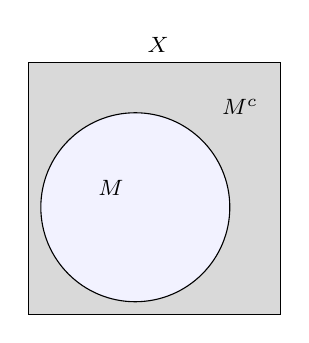
\begin{tikzpicture}[scale=0.8]
\def\firstcircle{(-0.3,-0.3) circle (1.5cm)}
\def\secondcircle{(-2,-2) rectangle ++(4,4)}
    \draw \secondcircle[fill=black!15] node at(1.3,1.3) {\begin{footnotesize} $M^c$ \end{footnotesize}};
    \node[anchor=south] at (current bounding box.north) {\begin{footnotesize} $X$\end{footnotesize}};
        \begin{scope}
        %\clip \firstcircle;
        \draw[fill=blue!5!white] \firstcircle node at(-0.75,0) {\begin{footnotesize} $M$ \end{footnotesize}};
        \secondcircle;
    \end{scope}
\end{tikzpicture} 
  \end{minipage}
%\end{figure}
\end{Definition}

\white{3cm}{}

\begin{Definition}{Product set}
 The \defi{Cartesian product} of two sets $A,B$ is
 given as the set of all \defi{pairs} (two elements with order):
 	$$
 		A \times B
 		:=  \{ (a,b) : a \in A, b \in B\}
 	$$
 	\begin{center}
 \includegraphics[width=0.3\linewidth]{pics/Cartesian2}	
 	\end{center}  
\vskip-2ex
\hfill {\tiny{(Source of the picture: Author Quartl - Wikipedia)}}
 \vskip2ex
 In the same sense, for sets $A_1, \ldots, A_n$
 the set of all \defi{$n$-tupels} is defined:
  	$$
 		A_1 \times \cdots \times
 		A_n
 		:=  \{ (a_1,\ldots, a_n) : a_1 \in A_1, \ldots, a_n \in A_n\}
 	$$
\end{Definition}


\white{3cm}{}

\begin{exercise}{Which statements are correct?}
\[
\false{\{1,3\} \cup \{2,4\} = \{1,2,4\}}, \qquad
%\corr{\{1,2,4\} \cup \{1,3,5\} = [5]}, \qquad
\corr{\{1,2\}\cup\{3,4\} = \{3,2,4,2,1\}},\qquad
\corr{\N \cup \Z = \Z}.
\]
\[
\corr{\{1,2,4\} \cap \{3,4,5\} = \{4\}}, \qquad
\corr{\{1,3\} \cap \{2,4\} = \varnothing}, \qquad
%\corr{[3] \cap [5] = [3]}, \qquad
\false{\N \cap \Z = \N_0}.
\]
\[
\false{\{1,2,4\} \setminus \{3,4,5\} = \{1\}}, \qquad
%\corr{[5] \setminus [3] = \{4,5\}}, \qquad
%\false{[3] \setminus [5] = \{1,2,3\}}.
\corr{\N_0\setminus\N=\{0\}},\qquad
\corr{\N\setminus\Z=\varnothing}.
\]
%\[
%\corr{[3,5]\cup[5,7] = [3,7]}, \qquad
%\false{[3,5]\cup(5,7) = (3,7)}, \qquad
%\corr{[3,5)\cup(5,7) = [3,7)\setminus \{5\}}.
%\]
\[
\false{\Z \setminus \N = \{-x\st x\in\N\}}, \qquad
\corr{\N \subset \N_0}, \qquad
%\igno{\N_0 \subset \Z, \qquad \Q \subset \R}
\false{\Z \subset \N_0}, \qquad
\corr{(\Z\setminus \Q) \subset \N}.
\]
\[
\corr{\N\subset\N}, \qquad
\corr{-3\in\Z\setminus\N_0}, \qquad
\corr{\tfrac37\in\Q\setminus\Z},\qquad
\corr{\sqrt{2}\in\R\setminus\Q},
\]
\igno{
\[
\text{Wenn $n\in\N$, dann $[n]= [1,n]\cap\N$.}
\]
}
%(Antwort: Die \textit{falschen} Aussagen sind durchgestrichen.)
\end{exercise}
%
\white{3.5cm}{}
%
~\\[-5em]
%\igno{
\begin{exercise}{}
Which claims are correct? Prove or give a counterexample.
\pres{Here, we solve one exercise in detail!}
\begin{abc}
%\item Wenn $n\in\N$, dann $[n]= [1,n]\cap\N$. 
\item $(\Q\setminus \R) \subset \N_0$. 
\white{30mm}{}
\item Let $A,B,C$ be three sets. Then one has
$A\cup (B\cap C) = (A\cup B) \cap C$.
\white{40mm}{}
\item Let $A,B,C$ be three sets. Then one has
$A\cap (B\cap C) = (A\cap B) \cap C$.
\white{30mm}{}
\item Let $A,B,C$ be three sets. Then one has
$A\setminus (B\cup C) = (A\setminus B) \cap (A\setminus C)$.
\white{50mm}{}
\end{abc}
\end{exercise}

\begin{exercise}{}
Describe the following sets and calculate its cardinalities:
\begin{abc}
\item $X_1:= \{ x\in\N \st \exists a, b\in \{1,2,3\} \text{ with } x=a-b \}$ \white{30mm}{}
\item $X_2:= \{ (a-b) \st a, b\in \{1,2,3\} \}$ \white{30mm}{}
\item $X_3:= \{ |a-b| \st a, b\in \{1,2,3\} \}$ \white{30mm}{}
\item $X_4:= \{1,...,20\} \setminus \{ n\in\N \st 
\exists a,b\in\N \text{ with } 2\le a \text{ and } 2\le b \text{ and } n=a\cdot b  \}$.\white{30mm}{}
\item $X_5:= \{ S \st S\subset \{1,2,3\} \}$.\white{20mm}{}
\end{abc}
\end{exercise}

%\begin{aufgabe}{}
%Es sei $n\in\N$. Wir definieren verschiedene Mengen, die von dem Parameter $n$ abhängen.
%Beschreiben Sie die folgenden Mengen und berechnen Sie ihre Kardinalität, jeweils in Abhängigkeit von $n$.\\
%a) $A_n:= [1]\cup [2] \cup \ldots \cup [n]$.\\
%b) $B_n:= [1]\cap [2] \cap \ldots \cap [n]$.\\
%c) $C_n:= \{ S \st S\subset [n] \}$.
%\end{aufgabe}
%